\documentclass{article}
\usepackage[utf8]{inputenc}
\usepackage[spanish,activeacute]{babel}
\usepackage[a4paper,top=3cm,bottom=2cm,left=3cm,right=3cm,marginparwidth=1.75cm]{geometry}
\usepackage{graphicx}
\usepackage[colorinlistoftodos]{todonotes}
\usepackage[colorlinks=true, allcolors=blue]{hyperref}
\usepackage {url}

\title{Documento Escrito \\Proyecto 2\\ Agencia de Automóviles en Java}
\author{Riaño Enriquez Donovan \\ Tapia Escobar José Alejandro\\Villaseñor Maulión Juan Luis}
\begin{document}
\maketitle 
\begin{flushleft}
Profesor: Tista García Edgar \newline \newline
Materia: Programación Orientada a Objetos \newline \newline
Semestre $2019-2$
\end{flushleft}
\clearpage

\begin{center}
\section{Objetivos}
\end{center}
\begin{itemize}
\item Que el alumno ponga en práctica todos los conceptos vistos a lo largo del curso en una aplicación real
\item Que el alumno fortalezca sus habilidades la programación orientada a objetos.
\item  Que el alumno fortalezca sus habilidades en trabajo en equipo.
\end{itemize}

\subsection{Objetivos Generales}
Nuestro Objetivo principal es pasar POO, pues los 3 somos recursadores de la materia y no nos gustaría ser ASDRIS, así como además tenernos paciencia,consideración y apoyo como equipo,porque  en un trabajo nos tocará trabajar con personas que a lo mejor no son tanto de nuestro agrado pero se tiene que realizar a fin de cuentas.

Como equipo tenemos la meta de entregar un proyecto bastante completo, a lo mejor no será la mejor agencia de autos, pero para nosotros será la mejor por la dedicación y empleo de tiempo que invertimos en él. Mantenemos el propósito de hacer un muy buen trabajo para superarnos también a nosotros mismos con nuestras propias expectativas.

\begin{center}
\section{Introducción}
\end{center}

El presente informe... nah, olvidelo xd.\newline

Para este proyecto cabe destacar que nosotros presentamos esta propuesta y si no llega a salir será nuestra propia muerte. El uso de la programación orientada a objetos es bastante útil, porque a la hora de elaborar nuestro código en vez de tener lineas por todas partes, con la POO es más fácil de ver errores, así como además poder ir agregando funcionalidades poco a poco sin que el demás código sufra muchos daños, que básicamente fue lo fuimos implementando.\newline

Planteamos y obviamente escogimos esta propuesta porque toca muchos puntos de los vistos en todo el curso, inclusive más con la cuestión de las interfaces gráficas. En cuestión de conceptos tocamos temas desde la instanciacón de clases y modificadores de acceso hasta temas como el posible manejo de hilos y de patrones de diseño.\newline

En los siguientes puntos describiremos un poco más detalladamente como fue que logramos nuestra implementación en cada tema que nos toco trabajar.\newline

\begin{center}
\section{Investigación Teórica}\cite{Mar}, \cite{dea}, \cite{kol}, \cite{ora}
\end{center}

\subsection{Colecciones}

Las colecciones son métodos proporcionados por el lenguaje Java que sirven para el uso más sencillo sobre Listas(tema visto en EDA I). Las colecciones son el agrupamiento de la información que tiene elementos o características  
(consecuentes o coherentes) similares.

Realmente aquí no utilizamos nada de colecciones por falta de tiempo pero si lo consideramos.

\subsection{Uso de Paquetes}

El uso de paquetes es empleado para no tener muchas clases en un mismo directorio y mantener un orden lógico de clases en el programa.\newline
Se apoya del razonamiento modificadores de acceso, no dar más acceso de información a las clases del que deben emplear.

\subsection{Modificadores de Acceso}

Los modificadores de Acceso sirven para poder encapsular mejor nuestros atributos. La razón principal de ellos es la correcta implementación de sus atributos 
y métodos que lo definen, para que de esta manera las clases tengan la comunicación necesaria de los elementos que necesitan y de cuales no.\newline

Para los modificadores de acceso en cuestión de las imágenes los labels, frames, etc, decidimos mantenerlos privados por las cuestiones
de que las demás clases no necesitan saber sus implementaciones. Para el friendly en la parte de la interfaz para que el main puediese ver bien
la instanciación.\newline

Y para el público para la interfaz y las clases abstractas, pues por definición deben de ser así.

\subsection{Documentación del Código con JavaDoc}

Javadoc es una herramienta proporcionada por el Lenguaje de programación Java que nos permite hacer una documentación ideal de nuestro código, tiene métodos prestablecidos. La manera en que la documentación se genera es con archivos html, donde directamente al abrirlos se pueden ver en cualquier navegador web. 
También es una razón legible y sencilla de realizar lo que a veces demora más tiempo.  La información sobre el código hecho se maneja con el API de Java.\newline

El javadoc lo realizamos y lo utilizamos para:
\begin{itemize}
\item[$*$] Atributos
\item[$*$] Métodos
\item[$*$] Autores
\item[$*$] Clases
%\item[$*$] Paquetes
\item[$*$] Funcionamiento del código

Donde no tratamos que fuera de lo más detallado pero si que supiera que es lo que se estaba relizando y porque decidimos realizarlo de esa manera.
\end{itemize}

\subsection{Herencia y polimorfismo}

En el proyecto involucramos indirectamenete ambas, pero más la herencia para la cuestión de las clases abstractas para hacer los métodos necesarios
a un nivel más particular de cada clase de automóvil.

\subsubsection{Herencia}

Es la división que se hace en una clase para establecer sub clases a partir de ella.\\
La propiedad de la herencia modela el hecho de que los objetos se definen o se comportan en modelos jerárquicos.\\
La jerarquía se establece desde el punto de vista del modelado se denomina relación de generalización ``es-un''.

\subsubsection{Polimorfismo}

Permite a una operación tener el mismo nombre en clases diferentes y que actúe de modo distinto en cada una de ellas.\\
También los objetos pueden responder de diferente manera al mismo mensaje

\subsection{Clases Abstractas e Interfaces}

Las clases Abstractas e Interfaces nos ayudan generalizar información. Genelizan aspectos comunes como atributos y características de los objetos de un problema, para ahorrar código redundante. Los atributos y métodos que se definan en ellos tienen que ser ``publicos'' y para el caso de las interfaces ``final'', pues estos métodos no se pueden redefinir.\newline

Solo empleamos una sola clase(Auto), la cual tenía cuatro métodos comunes de un automóvil(haciendo su abstracción) y son:
\begin{enumerate}
\item Marca
\item Modelo
\item Año
\item Serial
\end{enumerate}

Los cuales a su vez estan conectados con tres clases abstractas(HashBack,Lujo,Van), por ser métodos abstractos y a su vez puedan heredar clases(AutoHash,AutoLujo,AutoVan).

\subsection{Uso de Excepciones}

Las excepciones son ``situaciones'' que la máquina virtual de Java no detecta en tiempo de compilación.\newline

Estas pueden ser verificadas o no. Las verificadas son situaciones que se presentan a la hora de encontrar un archivo o una conexión a una base de datos de la cual necesitamos extraer información de ella. Las no verificadas son las que en tiempo de ejecución ocasionan problemas ya sea instrucciones del programador o por el mal ingreso de datos del usuario.\newline

Para el manejo de excepciones incluimos principalmente:\textit{RuntimeException, FileNotFoundException,} \textit{IOException}.\newline
\newline En el caso de \textit{RunTime} en el menú, pues si el usuario es descuidado no ingresaba una opción numérica entera al programa, la excepción la atrapaba y mandaba un mensaje de tipo de dato inválido.\newline
\newline \textit{FileNotFoundException} así como \textit{IOException} se implementaron para el manejo de archivos, en caso de que el archivo este corrupto o no se encuentre, puesto que  al ser ambas Excepciones verificadas, el compilador nos indicaba que debiamos incluirlas.

\subsection{Manejo de Archivos}

En el caso del manejo de archivos no podía ser posible sin la inclusión de excepciones, como describimos en el anterior punto.\newline
El manejo de Archivos se hace a través de flujos en Java (Streams), que permiten que el propio lenguaje pueda obtener información
 o para el manejo de la información en archivos fluya. \newline
En el manejo de archivos podemos afirmar que el manejo principal fue en los login, porque creamos 4 archivos de texto plano, los cuales tenían la función de
almacenar la información de usuarios, administradores y sus contraseñas, y a su vez en el programa este los utilizó para leer la información y validar con lo que el usuario
 en tiempo de compilación estaba ingresando.\newline
Además otro aspecto a considerar para el manejo de los archivos es el uso de las imágenes, pues estas también lo son, pero para su vista lo describiremos en el siguiente apartado.

\subsection{Manejo de Imágenes}

En cuestión del manejo de las imágenes incluimos las bibliotecas de \textit{javax.swing(JFrame, JPanel, JLabel, JImageIcon)}, las cuales nos permitieron a través de interfaz gráfica
 poder abrir las imágenes y poder cerrarlas cuando el usuario guste.\newline

Estas a su vez forma parte de la interfaz gráfica, y sin ellas no hubieramos podido abrir las imágenes de los autos. Al principio fue difícil de manipular, pues los ejemplos eran
más elaborados para clases más específicas o para abrir una imagen en sí, por lo que hacer la implementación para todas no fue de lo más sencillo.
\subsection{Diagramas UML}

La diagramación UML (Unified Modeling Language) es útil y es común a cualquier lenguaje orientado a objetos. Con la diagramación UML podemos modelar un problema físico a un modelo computacional a través de objetos. 
Los diagramas UML nos permiten abstraer un problema, así como hacer una correcta descripcióon del problema, ignorando detalles no importantes, facilitando el objeto a modelar.
Para los Diagramas UML utilizamos el software dia, el cual nos permitió hacer los diagramas de cada clase, así como además las conexiones de las clases.\newline

Considerando la redefinición de las clases nuestro diagrama UML cambio, este  diagrama era antes de la interfaz gráfica


\begin{itemize}
\item Relaciones de Depencia(Ejemplo: Login-AgenciaDeAutos)
\item Relaciones de Generalización(Ejemplo: AutoLujo-Lujo)
\item Relaciones de Realización(Ejemplo: Auto-Lujo-AutoLujo)
%\item Relaciones de Agregación y composición()
\end{itemize}


\begin{figure}
\centering
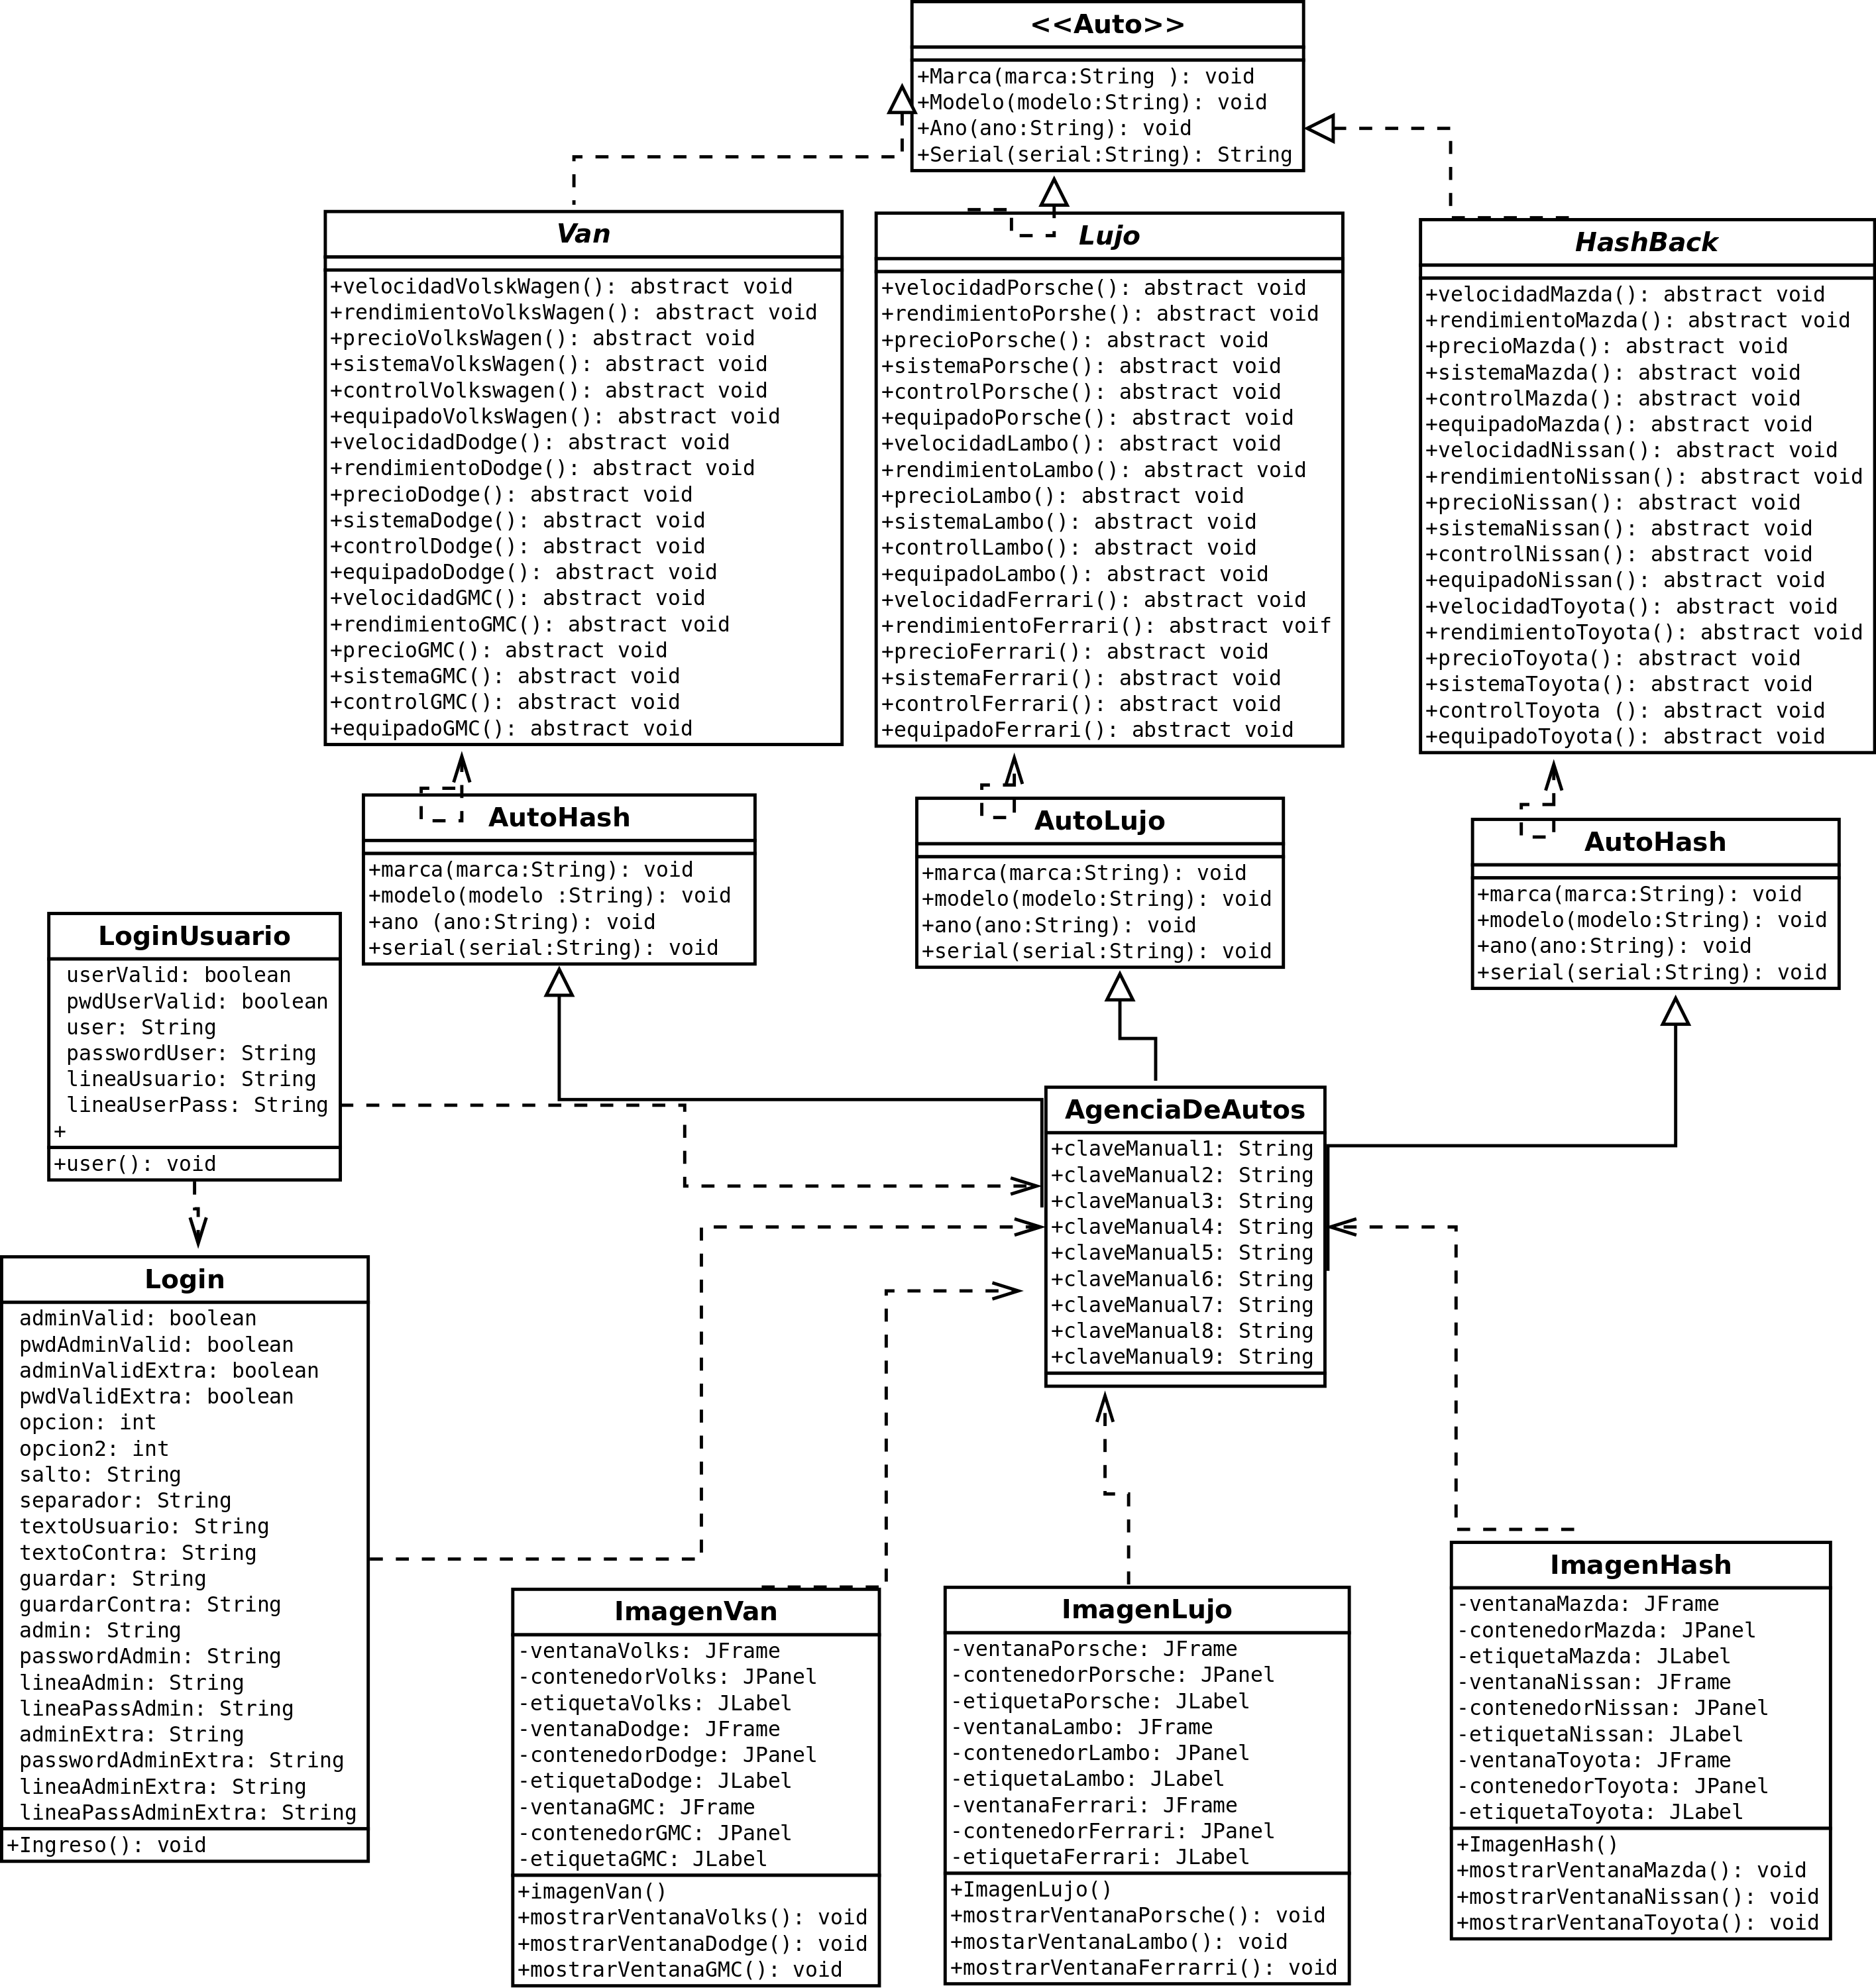
\includegraphics[width=0.5\textwidth]{DiagramasUML/Diagrama1.png}
\caption{\label{fig:tesla}Diagrama UML AgenciaDeCarros}
\end{figure}
\clearpage

Y después de la redefinición de esta quedó asi

\begin{figure}
\centering
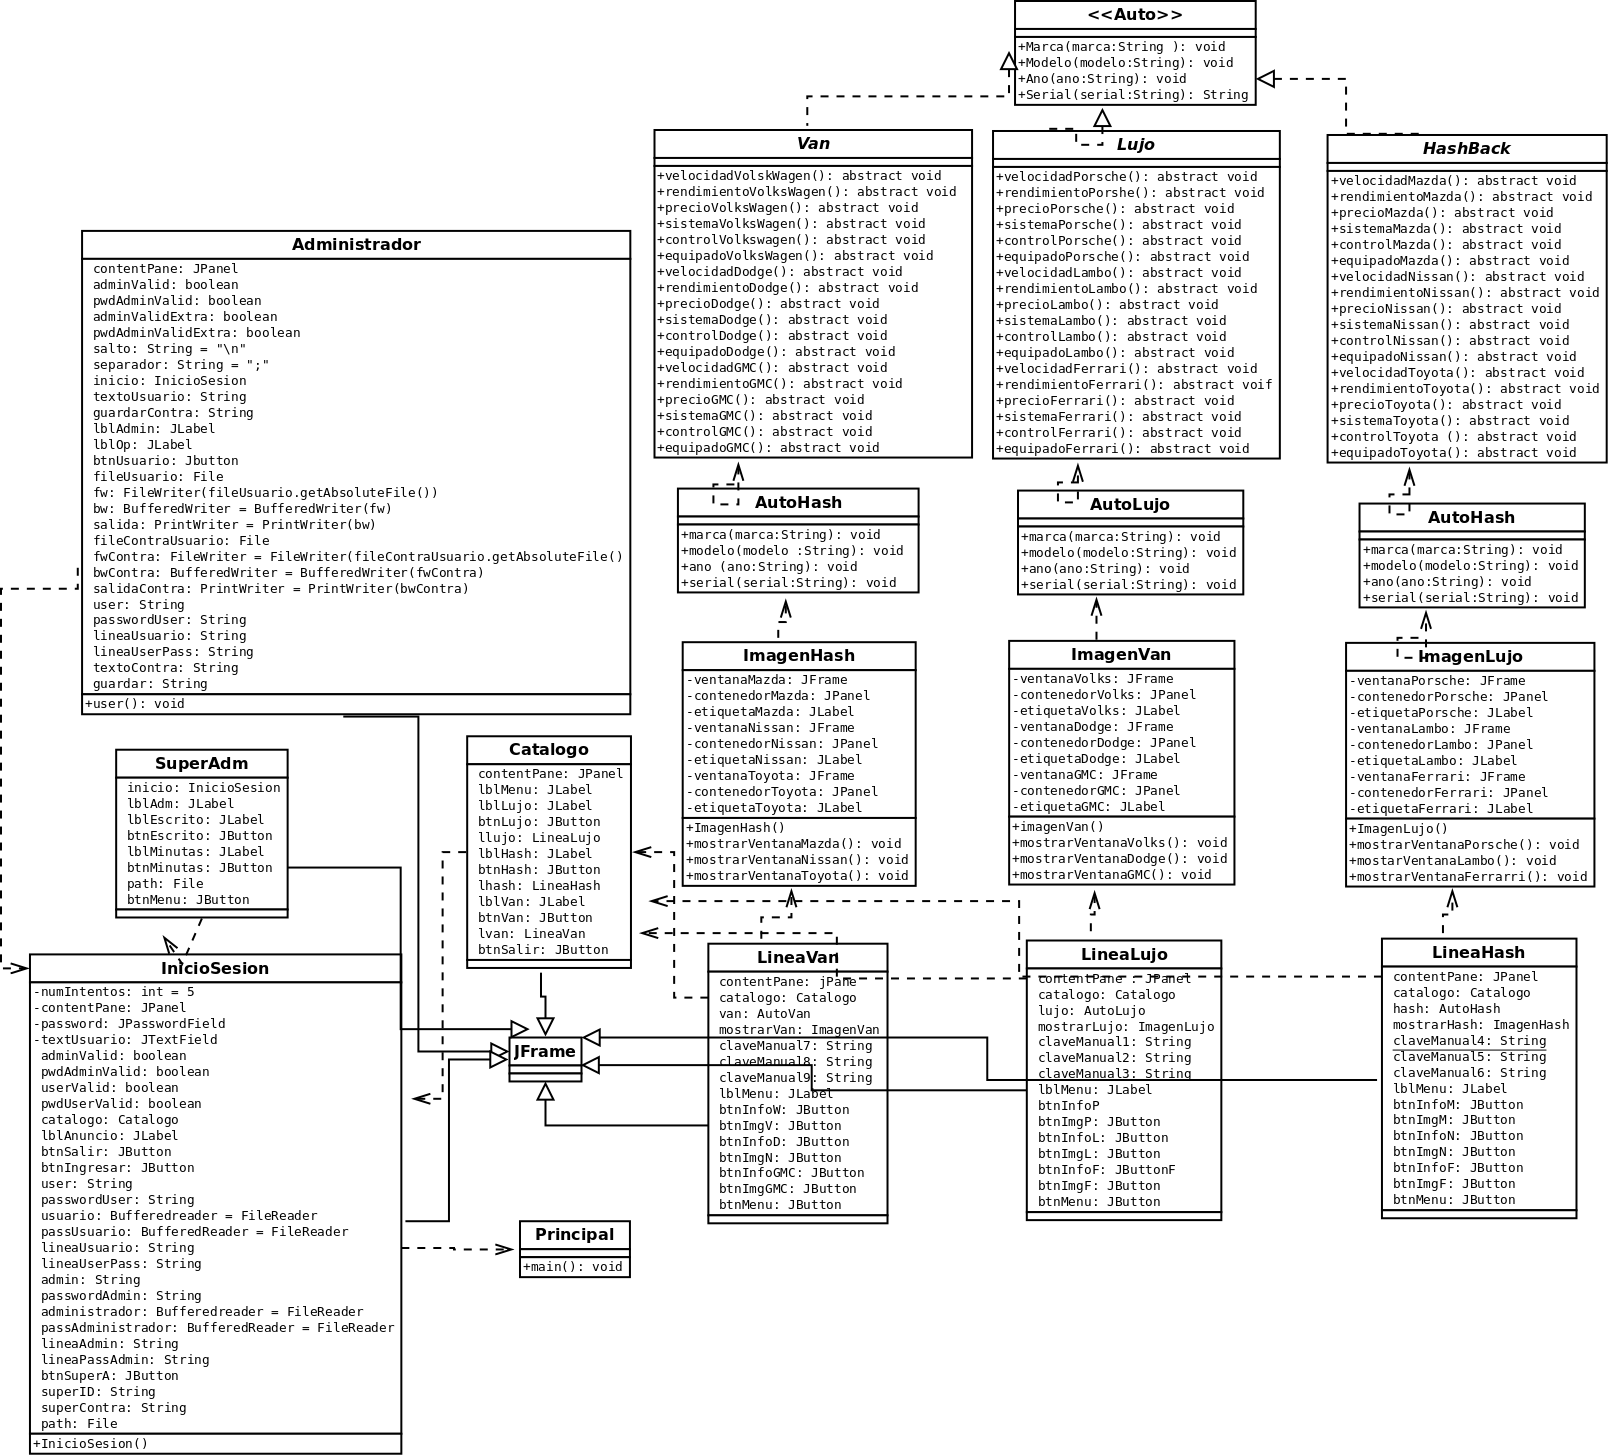
\includegraphics[width=0.5\textwidth]{DiagramasUML/Diagrama2.png}
\caption{\label{fig:tesla}Diagrama UML Principal}
\end{figure}


\subsection{Interfaz Gráfica}

La interfaz Gráfica es una forma más agradable e intuitiva para mostrar la información al usuario, donde de la misma manera es más sencilla su 
navegación.\newline

Para la Interfaz grafica lo mas complicado fue tenerla que haber realizado dos veces, la primera
fue por medio del ID Netbeans ya que al momento de exportar ese codigo y quererlo manejar por
medio de Sublime Tex el codigo no era compilado de manera correcta, a pesar de no existir ningun
error.

Al no poder conseguir conectar la interfaz al codigo de logica del trabajo, desicimos volver a crear
la interfaz por medio de fracmetos que ya teniamos de forma manual en Sublime, y ahí nos
enfrentamos a un segundo problema (el redefiniemto de clases) ya que teniamos problemas con el
metodo principal main, asi que decidimos hacer lo siguiente:

\begin{itemize}
\item  Primero creamos la clase inicio de sesión la cual solicitaba al usuario una cuenta y una
contraseña, ademas de distintos botones que permitian el acceso al administrador y al
super administrador cada uno con diferentes tareas, hasta ese punto todo iba bien,
decidimos crear una clase principal con el método main aparte de la clase ya mencionada
para solo instanciar el método dentro del main y mandarlo a llamar.

\item Cuando creamos la ventana de administrador y super administrador decidimos que ambos
tuvieran un botón especial el cual permitiera devolver a dichos empleados a la ventana
principal de la interfaz, esto se acordo a referente a una posible situación de que alguno de
los dos quisiera volver a repetir sus tareas específicas mas de una vez

\item El boton de ingresar permite la acción siguiente del usuario, es decir mostrar el menú de los
distintos tipos de auto (Lujo, Van y HatchBack) y, a su vez, cada uno de ellos cuenta con un
botón para ingresar al catálogo específico de distinta línea de modelo, nuevamente al ingresar
de (MENU -& gt; CATALOGO) el botón permite el retorno de (CATALOGO-&gt;MENU) pero el
menú de autos ya no puede retornar al menú principal esto quiere decir que una vez el
usuario haya accedido al meu de autos este solo podra navegar dentro de ese menú y sus
distintos catalogos una vez terminado de visualizar cada uno el usuario tendra la opcion de
salir de la interfaz

\end{itemize}


\begin{center}
\section{Conclusiones}
\end{center}

En general cumplimos con los aspectos tocados del curso y del proyecto. Los aspectos que hicieron falta fueron:\newline
\begin{itemize}
\item Paquetes:
Referente al manejo de paquetes tuvimos una cierta complicacion que tuvo que ver mas que nada con el ide para trabajr el proyecto, nos referimos a sublime y a Netbeans, ya que cuando creabamos la gerarquia de paquetes, en Netbeans al momento de correr el codigo ciertas adaptaciones que habiamos creado especialmente para nuestro codigo no eran detectadas por el ide.

Y en el caso de sublime los paquetes no eran reconocidos del todo, a pesar de haber generado una importacion y un uso de los mismos paquetes correctamente.

El equipo decidio optar por el hecho de NO realizar la utilizacion de paquete para no modificar los aspectos de punto especial que nostros mismo ideamos.

\item En el caso de la interfaz hizo falta realizar la conexión completa con ciertas ventanas para que pudiesen volver al menu principal
\end{itemize}

\newline Los aspectos en los que cumplimos fueron:

\begin{enumerate}
\item Nuestro desempeño general a lo largo del proyecto fue satisfactorio y favorecedor ya que como equipo supimos adaptarnos de la mejor manera y conseguimos que los conocimientos de cada uno se vieran reflejados en el proyecto, ademas de cumplir la mayor de metas que nostros mismos nos fijamos

\item Cumplimos referente al uso de Interfasce para mandar a llamar los atributos mas especificos  referente a los autos 

\item Supimos realizar la creacion de clases que heredaban de otra utilizando el extends y el implements ya que tambien derivaban de una una interfaz (ademas del metodo super para utilizar los metodos de la clase padre)

\item Utilizamos el @Override para indicar que ese meto era reutilizado en otras clases (buenas practicas)

\item Realizamos la creacion de clases abstractas para indicar los metodos mas especificos de cada auto, marca y linea.

\item Se realizaron ventanas especiales para el manejo de la interfaz grafica utilizando la clase derivada JFrame la cual nos permite el manejo de los swings en java junto con todos los aspectos especificos que utilizamos como el JLabel, JOptionPane, JButton, entre otros

\item Realizamos el manejo de excepciones correctamente

\end{enumerate}



\subsection{Conclusiones Riaño Enriquez Donovan}

Fue un buen reto que personalmente me puse, porque yo fui el de la idea principalmente de este proyecto. Mis aspectos a considerar fueron los de mantener un equipo unido, comunicado y a su vez que entregará resultados.\newline

En cuestión de código fui el que realizó la mayor implementación, así como la estructura general, jerárquica y lógica de clases para el funcionamiento del código.\newline

Tengo que admitir que la verdad no sabía en un principio sobre como iba a cumplir con la propuesta en sí, pero muy dentro de mí si sabía que lo iba a lograr de un modo u otro, y que esto traería como consecuencia un mejor desempeño programando y de superación de mis expectativas como alumno.

\subsection{Conclusiones Tapia Escobar Alejandro}

El proyecto fue algo muy bueno que permitio el hecho de poner a pruba todos
nuestros conocimientos vistos en clase en una sola super practica. Creo que en lo
personal me todo un excelente equipo ya que cada uno manejabamos algo en
especial que nos funciono para la creacion del proyecto y ese mismo conocimiento
lo pudimos transmitir entre nosotros sin ninguna complicacion. Mi parte fue la
logica de interfaz, y en realidad fue un gran reto realizarla de forma manual y
acoplarme al codigo de Riaño, ya que para mi hubiese sido mas sencillo primero
armar un cascaron y despues su logica pero al final cumplimos con la mayoria de
las metas propuestas.

\subsection{Conclusiones Villaseñor Maulión Juan Luis}

Puedo concluir que este proyecto final fue un trabajo difícil porque se ponen a prueba todos los conocimientos obtenidos a lo largo del semestre. Observé que el paradigma orientado a objetos es bastante complicado porque trabajar con todos los temas en conjunto puede ser algo confuso. 
En el proyecto realice el Javadoc que para empezar tuve que investigar que era el Javadoc porque jamás había trabajado con eso, no es complicado pero siempre enfrentarse a un tema desconocido puede ser un reto a lograr. Fue algo similar a lo que me pasó con LaTex, jamás había utilizado LaTex en mi vida pero después de un tiempo de estar practicando te das cuenta de la facilidad de usar LaTex y todas las ventajas que te ofrece este sistema de composición de textos científicos.
En general conformamos un equipo que se comunicaba bastante bien, esto ayudó a que muchos de los objetivos del proyecto se lograran de una forma satisfactoria y cada quien se llevara un aprendizaje importante de todos los temas del curso. 


\begin{thebibliography}{x}
  
  \bibitem{Mar} Martín, Antonio. Programador Certificado Java 2.Segunda Edición.México. Alfaomega Grupo Editor,2008.
  \bibitem{dea} Dean John and Dean Raymond. Introducción a la programación con Java.Primera Edición.México.Mc-Graw Hill, 2009.
  \bibitem {kol} Barnes David and Kölling Michael. Programación Orientada a Objetos con Java. Tercera edición. Madrid. Pearson Education, 2007. 
  \bibitem {ora} Varios Autores. How to Write Doc Comments for the Javadoc Tool. Oracle. \url{https://www.oracle.com/technetwork/articles/javase/index-137868.html} visitado: 21-05-2019.

\end{thebibliography}

En también  utilizamos las láminas de los temas vistos en clase, así como el parafraseo de los conceptos.


\bibliographystyle{abbrv}

\end{document}
